\section{314 --- Binary Tree Vertical Order Traversal}

\textbf{Medium}

Given a binary tree, return the vertical order traversal of its nodes' values. (ie, from top to bottom, column by column).

If two nodes are in the same row and column, the order should be from left to right.

\paragraph{Examples 1:}
\begin{flushleft}
\textbf{Input}: 

\begin{figure}[H]
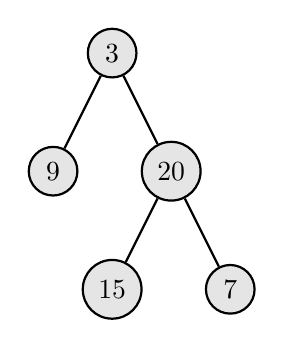
\begin{tikzpicture}
[every node/.style={draw, circle, fill=gray!20!, minimum size=5mm},
thick]
\node{3}
child{node{9}}
child{node{20} child{node{15}} child{node{7}}};
\end{tikzpicture}
\end{figure}



\textbf{Output}:

\fcj{[[9], [3,15], [20], [7]]}
\end{flushleft}
\paragraph{Examples 2:}
\begin{flushleft}
\textbf{Input}: 

\begin{figure}[H]
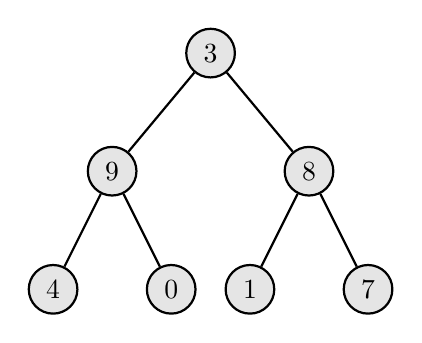
\begin{tikzpicture}
[every node/.style={draw, circle, fill=gray!20!, minimum size=5mm},
level 1/.style={sibling distance=25mm},
level 2/.style={sibling distance=15mm},
thick]
\node{3}
child{node{9} child{node{4}} child{node{0}}}
child{node{8} child{node{1}} child{node{7}}};
\end{tikzpicture}
\end{figure}

\textbf{Output}:

\fcj{[[4], [9], [3,0,1], [8], [7]]}



\end{flushleft}

\subsection{BFS}
Using level traversal, mark each node with a unique number. 

The number of the left child is current node's number minus 1 and the right child is plus 1.

Then we group the nodes with same numbers.


\setcounter{lstlisting}{0}
\begin{lstlisting}[style=customc, caption={BFS}]
vector<vector<int>> verticalOrder( TreeNode* root )
{
    if( !root )
    {
        return {};
    }
    queue<pair<int, TreeNode*>> q;
    q.emplace( 0, root );
    map<int, vector<int>> m;
    while( !q.empty() )
    {
        auto [id, t] = q.front();
        q.pop();
        //add to map
        m[id].push_back( t->val );
        if( t->left )
        {
            q.emplace( id - 1, t->left );
        }
        if( t->right )
        {
            q.emplace( id + 1, t->right );
        }
    }
    //copy data from map to output
    vector<vector<int>> ans;
    for( auto&[id, v] : m )
    {
        ans.emplace_back( begin( v ), end( v ) );
    }
    return ans;
}
\end{lstlisting}

\paragraph{Related Problems}
\begin{itemize}
\item \textbf{102. Binary Tree Level Order Traversal}
\end{itemize}